%%% Sekce – Správa nákupního košíku
%%%%% Wording: ✅
%%%%% Styling: ✅
%%%%% References: ✅
%%% --------------------------------------------------------------
\section{Správa košíku}
\label{sec:implementace-kosik}
Druhým hlavním prvkem této aplikace je správa nákupního košíku.
Tento prvek umožňuje uživatelům přidávat, odebírat nebo vyměňovat vstupenky, které si vybrali z mapy sedadel.
Správa košíku je pro aplikaci klíčová, jelikož slouží jako most mezi interaktivní mapou sedadel, procesem rezervace a konečné platby.

%%% Podsekce – Kontext košíku
%%%%% Wording: ✅
%%%%% Styling: ✅
%%%%% References: ✅
%%% --------------------------------------------------------------
\begin{subsection}{Kontext košíku}
    \label{subsec:implementace-kosik-kontext}
    \foreign{State}, česky stav, košíku je spravován globálně v celé aplikaci pomocí kontextu.
    Toto zajišťuje \texttt{CartContext} komponenta, která obaluje celou aplikaci a poskytuje tak přístup a manipulaci se stavem košíku.
    Hlavní logika se odehrává v \texttt{useCart} hooku košíku, který vytváří instanci nákupního košíku, která obashuje stav a nabízí dostupné akce, kterými lze stav košíku měnit, jak lze vidět na diagramu~\ref{fig:cart-context-diagram}.

    \begin{figure}[H]
        \centering
        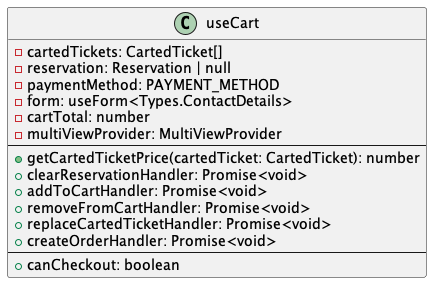
\includegraphics[width=0.6\textwidth]{\FIGDIR/diagrams/use-cart}
        \caption{Diagram \texttt{useCart} hooku}
        \label{fig:cart-context-diagram}
    \end{figure}
\end{subsection}

%%% Podsekce – Stav a funkce košíku
%%%%% Wording: ✅
%%%%% Styling: ✅
%%%%% References: ✅
%%% --------------------------------------------------------------
\begin{subsection}{Stav a funkce košíku}
    \label{subsec:implementace-kosik-stav}
    Z pohledu vstupenek a sedadel uchovává košík hlavně vstupenky, které jsou přidány do košíku.
    Tento stav je reprezentován polem objektů ve tvaru rozhraní zobrazeného v ukázce kódu~\ref{lst:carted-ticket}.

    \begin{listing}[H]
        \begin{minted}{typescript}
/**
 * CartedTicket type
 * @export
 */
export type CartedTicket = {
	/** unique carted ticket id */
	cartedTicketId: UUID;
	/** reference to the ticket received from API */
	ticket: VenueApiTypes.Ticket;
	/** reference to the specific seat */
	/** the Seat type received from API is extended with a specific category */
	/** also tickets array from the seat type is ommited as it does not make sense here */
	seat?: Extend<
		{
			category: VenueApiTypes.Category;
		},
		Omit<VenueApiTypes.Seat, 'tickets'>
	>;
};
        \end{minted}
        \caption{Rozhraní \texttt{CartedTicket}}
        \label{lst:carted-ticket}
    \end{listing}

    Košík, jak již bylo zmíněno, nabízí akce, kterými lze stav košíku měnit.
    Tyto akce, reprezentované tzv. \foreign{handlery}\footnote{\foreign{Handlery} jsou v tomto případě funkce vytvořené pomocí vlastního \texttt{useHandler} hooku, který je implementován v souboru \texttt{src/lib/hooks/useHandler.ts}.}, zahrnují především \texttt{addToCartHandler()}, \texttt{removeFromCartHandler()} a \texttt{replaceCartedTicketHandler()}.
    Také poskytuje metodu \texttt{getCartedTicketPrice()}, která vrací cenu konkrétní vstupenky v košíku na základě sedadla a kategorie vstupenky, jelikož cena vstupenky je definována kombinací její kategorie a vybraného sedadla.
    Implementace metody \texttt{getCartedTicketPrice()} je pro ilustraci uvedena v ukázce kódu~\ref{lst:get-carted-ticket-price}.

    \begin{listing}[H]
        \begin{minted}{typescript}
/** returns carted ticket price */
const getCartedTicketPrice = (cartedTicket: Types.CartedTicket) => {
	/** ticket without seat */
	if (!isDefined(cartedTicket.seat)) return cartedTicket.ticket.price;
	/** get ticket category */
	const ticketCategory = valOrThrow(
		cartedTicket.ticket.categories.find(({ categoryId }) => categoryId === cartedTicket.seat?.categoryId),
		`Ticket category not found for seat ${cartedTicket.seat.seatId}`,
	);
	/** return ticket category price */
	return ticketCategory.price;
};
        \end{minted}
        \caption{Implementace metody \texttt{getCartedTicketPrice()}}
        \label{lst:get-carted-ticket-price}
    \end{listing}

    V poslední řadě košík uchovává \foreign{memoizovanou}\footnote{\foreign{Memoizace} je optimalizacační technika, která ukládá výsledky volání funkce a při jejím opakovaném volání s týmiž parametry vrací uložený výsledek místo opětovného výpočtu.} hodnotu celkové ceny všech vstupenek v košíku, která je implementována jednoduše pomocí redukce pole vstupenek v košíku sečtením cen všech vstupenek prostřednictvím metody \texttt{getCartedTicketPrice} zmíněné výše.
\end{subsection}

%%% Podsekce – Vizualizace košíku
%%%%% Wording: ✅
%%%%% Styling: ✅
%%%%% References: ✅
%%% --------------------------------------------------------------
\begin{subsection}{Vizualizace košíku}
    \label{subsec:implementace-kosik-vizualizace}
    Košík je tímto již funkční, ale stále není zobrazen uživateli.
    Jeho zobrazení je zajištěno komponentou \texttt{Cart}, která zobrazuje stav košíku a poskytuje uživateli způsob interakce s ním.
    Jelikož prvním krokem celého nákupního procesu je výběr sedadla, není košík viditelný, dokud není vybráno sedadlo a vstupenka není přidána do košíku.
    Košík je pak zobrazen jako plovoucí prvek na pravé straně obrazovky, v případě desktopového zobrazení, a jako spodní list na mobilním zařízení, jak je navrženo v~\ref{subsec:narvh-ui-transformace-uzivatelskych-pribehu-nakupni-kosik}.
    Aktuální pohled na dosavadní implementaci košíku je zobrazen na obrázku~\ref{fig:seating-map-cart}.

    \begin{figure}[h]
        \centering
        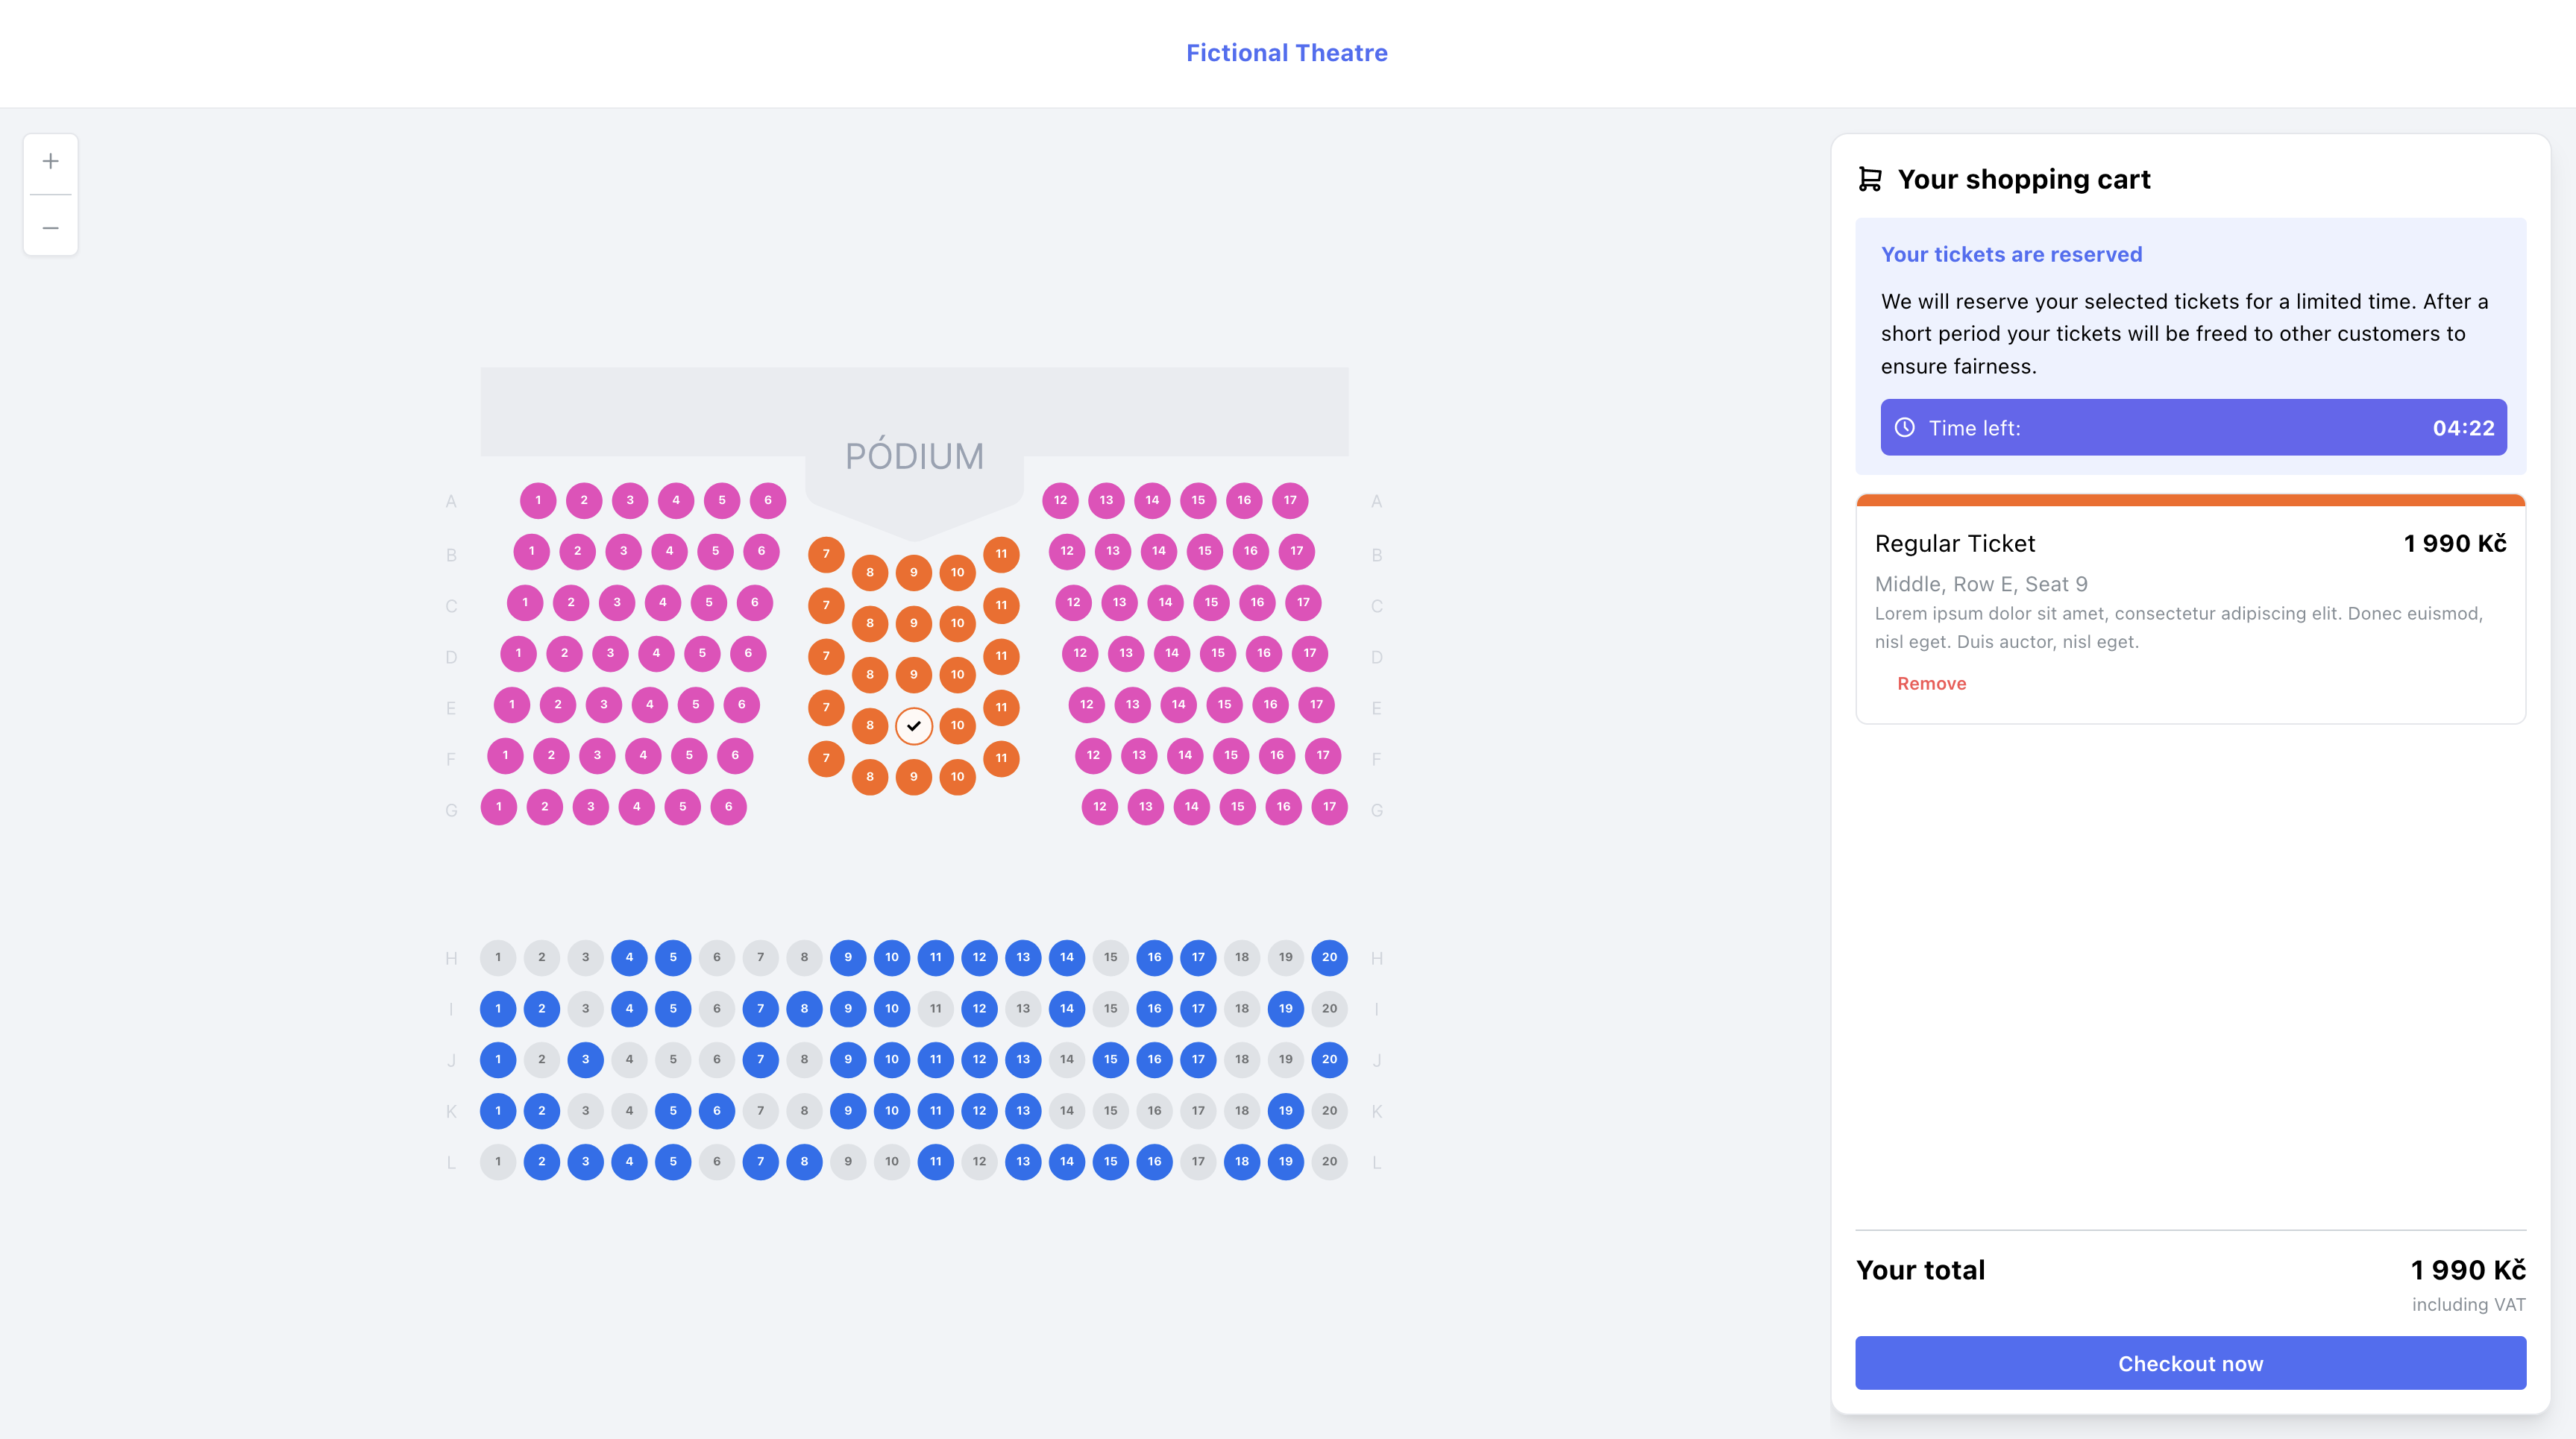
\includegraphics[width=\textwidth]{\FIGDIR/seating-map-cart}
        \caption{Snímek obrazovky košíku}
        \label{fig:seating-map-cart}
    \end{figure}
\end{subsection}

%%% Podsekce – Integrace API
%%%%% Wording: ✅
%%%%% Styling: ✅
%%%%% References: ✅
%%% --------------------------------------------------------------
\begin{subsection}{Integrace API}
    \label{subsec:implementace-kosik-api}
    Jelikož součástí této práce není implementace backendového systému, je stav košíku synchronizován s mock \ac{api}, aby se napodobila situace v reálné aplikaci.
    Kdykoli uživatel provede nějakou akci v košíku, je jeho stav aktualizován s malým zpožděním, aby se napodobila síťová latence reálného \ac{api}.
    Toho je dosaženo voláním asynchronní funkce, která vrací \foreign{promise}, který se vyřeší po nějaké specifikované době.
    V tomto případě se jedná o vlastní funkci \texttt{simulatedNetworkDelay()}, která je zobrazena v ukázce kódu~\ref{lst:simulated-network-delay} spolu se všemi ostatními použitými funkcemi.

    \begin{listing}[H]
        \begin{minted}{typescript}
/**
 * Simulates network delay
 * @param {"normal" | "heavy"} type
 * @return {Promise<void>}
 */
export const simulatedNetworkDelay = async (type: 'normal' | 'heavy' = 'normal') => {
	const delay = type === 'normal' ? 1000 : 5000;
	await fakePromise(DELAY_NETWORK ? randomIntBetween(delay * 0.25, delay) : 0);
};

/**
 * Resolves generated promise with optional value
 * @param {number} delay
 * @param {() => any} resolver
 * @param value
 * @returns {Promise<unknown>}
 */
export const fakePromise = (delay: number, resolver?: () => any, value?: any) =>
	new Promise((resolve) =>
		setTimeout(
			() => {
				resolver?.();
				resolve(value);
			},
			delay,
			value,
		),
	);

/**
 * Returns random integer from an interval
 * @param {number} min
 * @param {number} max
 * @return {number}
 */
export const randomIntBetween = (min: number, max: number): number => Math.floor(randomNumBetween(min, max));
        \end{minted}
        \caption{Implementace funkce \texttt{simulatedNetworkDelay() a její pomocné funkce}}
        \label{lst:simulated-network-delay}
    \end{listing}

    Užití funkce \texttt{simulatedNetworkDelay()} je pak zobrazeno v ukázce kódu~\ref{lst:remove-from-cart-handler}, která implementuje metodu \texttt{removeFromCartHandler}.

    \begin{listing}[H]
        \begin{minted}[highlightlines={9-10}]{typescript}
/** remove from cart handler */
const removeFromCartHandler = useHandler<Types.UseCart.RemoveFromCartCb>(
	async (cartedTicketId) => {
		/** clear reservation if last carted ticket */
		if (cartedTickets.length === 1) {
			console.log('[Cart] Removing last carted ticket, removing reservation...');
			await simulatedNetworkDelay();
			await clearReservationHandler.handler();
		}
		/** TODO: API should be called instead */
		await simulatedNetworkDelay();
		console.log('[Cart] Updating reserved cart');
		/** remove from cart */
		console.log('[Cart] Removing from cart:', cartedTicketId);
		_setCartedTickets((prev) => prev.filter(({ cartedTicketId: _cartedTicketId }) => _cartedTicketId !== cartedTicketId));
	},
	{
		deps: [cartedTickets],
	},
);
        \end{minted}
        \caption{Ukázka kódu implementující metodu \texttt{removeFromCartHandler()}}
        \label{lst:remove-from-cart-handler}
    \end{listing}

    Detaily zmíněné výše jsou jádrem logiky košíku.
    Jak se může zdát, logika košíku je poměrně jednoduchá, ale je zásadní pro funkčnost aplikace.
    V kódu výše na řádku 9 je podmíněné volání \texttt{clearReservationHandler()}, což je první náznak integrace rezervačního mechanismu do jádra košíku.
    Více o rezervaci a jejím mechanismu je popsáno v následující sekci.
\end{subsection}
